\documentclass[11pt]{article}
\setlength {\textwidth}{180mm} 
\setlength {\textheight}{260mm}
\topmargin=-35.00mm
\oddsidemargin=-10.00mm
\pagestyle{empty}


\usepackage[toc,page]{appendix}
\usepackage{amsmath, amssymb}
\usepackage{bm}% bold math
\usepackage{cancel, caption}
\usepackage{dcolumn}% Align table columns on decimal point
\usepackage{epsfig, epsf}
\usepackage{graphicx,fancyhdr,natbib,subfigure}
\usepackage{lscape, longtable}
\usepackage{hyperref,ifthen}
\usepackage{verbatim}
\usepackage{color}
\usepackage[usenames,dvipsnames]{xcolor}
\usepackage{listings}
%% http://en.wikibooks.org/wiki/LaTeX/Colors



%%%%%%%%%%%%%%%%%%%%%%%%%%%%%%%%%%%%%%%%%%%
%       define Journal abbreviations      %
%%%%%%%%%%%%%%%%%%%%%%%%%%%%%%%%%%%%%%%%%%%
\def\nat{Nat} \def\apjl{ApJ~Lett.} \def\apj{ApJ}
\def\apjs{ApJS} \def\aj{AJ} \def\mnras{MNRAS}
\def\prd{Phys.~Rev.~D} \def\prl{Phys.~Rev.~Lett.}
\def\plb{Phys.~Lett.~B} \def\jhep{JHEP} \def\nar{NewAR}
\def\npbps{NUC.~Phys.~B~Proc.~Suppl.} \def\prep{Phys.~Rep.}
\def\pasp{PASP} \def\aap{Astron.~\&~Astrophys.} \def\araa{ARA\&A}
\def\jcap{\ref@jnl{J. Cosmology Astropart. Phys.}}%
\def\physrep{Phys.~Rep.}

\newcommand{\preep}[1]{{\tt #1} }

%%%%%%%%%%%%%%%%%%%%%%%%%%%%%%%%%%%%%%%%%%%%%%%%%%%%%
%              define symbols                       %
%%%%%%%%%%%%%%%%%%%%%%%%%%%%%%%%%%%%%%%%%%%%%%%%%%%%%
\def \Mpc {~{\rm Mpc} }
\def \Om {\Omega_0}
\def \Omb {\Omega_{\rm b}}
\def \Omcdm {\Omega_{\rm CDM}}
\def \Omlam {\Omega_{\Lambda}}
\def \Omm {\Omega_{\rm m}}
\def \ho {H_0}
\def \qo {q_0}
\def \lo {\lambda_0}
\def \kms {{\rm ~km~s}^{-1}}
\def \kmsmpc {{\rm ~km~s}^{-1}~{\rm Mpc}^{-1}}
\def \hmpc{~\;h^{-1}~{\rm Mpc}} 
\def \hkpc{\;h^{-1}{\rm kpc}} 
\def \hmpcb{h^{-1}{\rm Mpc}}
\def \dif {{\rm d}}
\def \mlim {m_{\rm l}}
\def \bj {b_{\rm J}}
\def \mb {M_{\rm b_{\rm J}}}
\def \mg {M_{\rm g}}
\def \qso {_{\rm QSO}}
\def \lrg {_{\rm LRG}}
\def \gal {_{\rm gal}}
\def \xibar {\bar{\xi}}
\def \xis{\xi(s)}
\def \xisp{\xi(\sigma, \pi)}
\def \Xisig{\Xi(\sigma)}
\def \xir{\xi(r)}
\def \max {_{\rm max}}
\def \gsim { \lower .75ex \hbox{$\sim$} \llap{\raise .27ex \hbox{$>$}} }
\def \lsim { \lower .75ex \hbox{$\sim$} \llap{\raise .27ex \hbox{$<$}} }
\def \deg {^{\circ}}
%\def \sqdeg {\rm deg^{-2}}
\def \deltac {\delta_{\rm c}}
\def \mmin {M_{\rm min}}
\def \mbh  {M_{\rm BH}}
\def \mdh  {M_{\rm DH}}
\def \msun {M_{\odot}}
\def \z {_{\rm z}}
\def \edd {_{\rm Edd}}
\def \lin {_{\rm lin}}
\def \nonlin {_{\rm non-lin}}
\def \wrms {\langle w_{\rm z}^2\rangle^{1/2}}
\def \dc {\delta_{\rm c}}
\def \wp {w_{p}(\sigma)}
\def \PwrSp {\mathcal{P}(k)}
\def \DelSq {$\Delta^{2}(k)$}
\def \WMAP {{\it WMAP \,}}
\def \cobe {{\it COBE }}
\def \COBE {{\it COBE \;}}
\def \HST  {{\it HST \,\,}}
\def \Spitzer  {{\it Spitzer \,}}
\def \ATLAS {VST-AA$\Omega$ {\it ATLAS} }
\def \BEST   {{\tt best} }
\def \TARGET {{\tt target} }
\def \TQSO   {{\tt TARGET\_QSO}}
\def \HIZ    {{\tt TARGET\_HIZ}}
\def \FIRST  {{\tt TARGET\_FIRST}}
\def \zc {z_{\rm c}}
\def \zcz {z_{\rm c,0}}

\newcommand{\ltsim}{\raisebox{-0.6ex}{$\,\stackrel
        {\raisebox{-.2ex}{$\textstyle <$}}{\sim}\,$}}
\newcommand{\gtsim}{\raisebox{-0.6ex}{$\,\stackrel
        {\raisebox{-.2ex}{$\textstyle >$}}{\sim}\,$}}
\newcommand{\simlt}{\raisebox{-0.6ex}{$\,\stackrel
        {\raisebox{-.2ex}{$\textstyle <$}}{\sim}\,$}}
\newcommand{\simgt}{\raisebox{-0.6ex}{$\,\stackrel
        {\raisebox{-.2ex}{$\textstyle >$}}{\sim}\,$}}

\newcommand{\Msun}{M_\odot}
\newcommand{\Lsun}{L_\odot}
\newcommand{\lsun}{L_\odot}
\newcommand{\Mdot}{\dot M}

\newcommand{\sqdeg}{deg$^{-2}$}
\newcommand{\lya}{Ly$\alpha$\ }
%\newcommand{\lya}{Ly\,$\alpha$\ }
\newcommand{\lyaf}{Ly\,$\alpha$\ forest}
%\newcommand{\eg}{e.g.~}
%\newcommand{\etal}{et~al.~}
\newcommand{\lyb}{Ly$\beta$\ }
\newcommand{\cii}{C\,{\sc ii}\ }
\newcommand{\ciii}{C\,{\sc iii}]\ }
\newcommand{\civ}{C\,{\sc iv}\ }
\newcommand{\SiIV}{Si\,{\sc iv}\ }
\newcommand{\mgii}{Mg\,{\sc ii}\ }
\newcommand{\feii}{Fe\,{\sc ii}\ }
\newcommand{\feiii}{Fe\,{\sc iii}\ }
\newcommand{\caii}{Ca\,{\sc ii}\ }
\newcommand{\halpha}{H\,$\alpha$\ }
\newcommand{\hbeta}{H\,$\beta$\ }
\newcommand{\hgamma}{H\,$\gamma$\ }
\newcommand{\hdelta}{H\,$\delta$\ }
\newcommand{\oi}{[O\,{\sc i}]\ }
\newcommand{\oii}{[O\,{\sc ii}]\ }
\newcommand{\oiii}{[O\,{\sc iii}]\ }
\newcommand{\heii}{[He\,{\sc ii}]\ }
\newcommand{\nv}{N\,{\sc v}\ }
\newcommand{\nev}{Ne\,{\sc v}\ }
\newcommand{\neiii}{[Ne\,{\sc iii}]\ }
\newcommand{\aliii}{Al\,{\sc iii}\ }
\newcommand{\siiii}{Si\,{\sc iii}]\ }


%%%%%%%%%%%%%%%%%%%%%%%%%%%%%%%%%%%%%%%%%%%%%%%%%%%%%
%              define Listings                       %
%%%%%%%%%%%%%%%%%%%%%%%%%%%%%%%%%%%%%%%%%%%%%%%%%%%%%
\definecolor{dkgreen}{rgb}{0,0.6,0}
\definecolor{gray}{rgb}{0.5,0.5,0.5}
\definecolor{mauve}{rgb}{0.58,0,0.82}

\lstset{frame=tb,
  language=Python,
  aboveskip=3mm,
  belowskip=3mm,
  showstringspaces=false,
  columns=flexible,
  basicstyle={\small\ttfamily},
  numbers=none,
  numberstyle=\tiny\color{gray},
  keywordstyle=\color{blue},
  commentstyle=\color{dkgreen},
  stringstyle=\color{mauve},
  breaklines=true,
  breakatwhitespace=true,
  tabsize=3
}

\begin{document}

\title{A Glossary to some General (Astro)Physical terms}
\author{Nicholas P. Ross}
\date{\today}
\maketitle


\begin{abstract}
This is a simple document which will hopefully\/eventually be a pretty complete
list/glossary of various Astro)Physical terms and `what they mean'. There will 
be some overlap here with my other Research Notes, e.g. the Emission Line
document...
\end{abstract}

\section{A}
\section{B}
    \subsection{Bondi Accretion}
    % astro.physics.uiowa.edu/~kaaret/heastro10s/L12_agn.pdf
    AGN Accrete from the ISM, Via Bondi accretion:
    \begin{equation}
      \dot{M} \simeq (1.4\times10^{11} \rm{g/s}) \left( \frac{M}{M_{\Theta}} \right) \left( \frac{\rho}{10^{-24}\ \rm{g / cm^{3}}} \right)  \left( \frac{c_s}{10 \rm{km/s}} \right)^{-3}
    \end{equation}
    
    
    \subsection{BPT diagram}
    Straight from:\href{http://ned.ipac.caltech.edu/level5/Glossary/Essay_bpt.html}{Level 5 BPT}
    
    ``Baldwin, Phillips \& Terlevich'' (BPT) diagrams demonstrate how LINERs can be distinguished from normal H II regions and normal AGNs (Seyferts and QSOs) on the basis of their [O III] $\lambda$5007 / H$\beta$, [N II] $\lambda$6583 / H$\alpha$, and [S II] $\lambda \lambda$6716, 6731 / H$\alpha$ flux ratios. Here it is seen that the Seyfert 2s have high values of each ratio. H II regions define a locus of lower values which does not overlap with the region of parameter space occupied by the Seyferts. The LINERs can be distinguished from the Seyfert 2s by their low values of [O III] $\lambda$5007 / H$\beta$ relative to [N II] $\lambda$6583 / H$\alpha$, and from the H II regions by their larger values of [N II] $\lambda$6583 / H$\alpha$. 

    \begin{figure}
      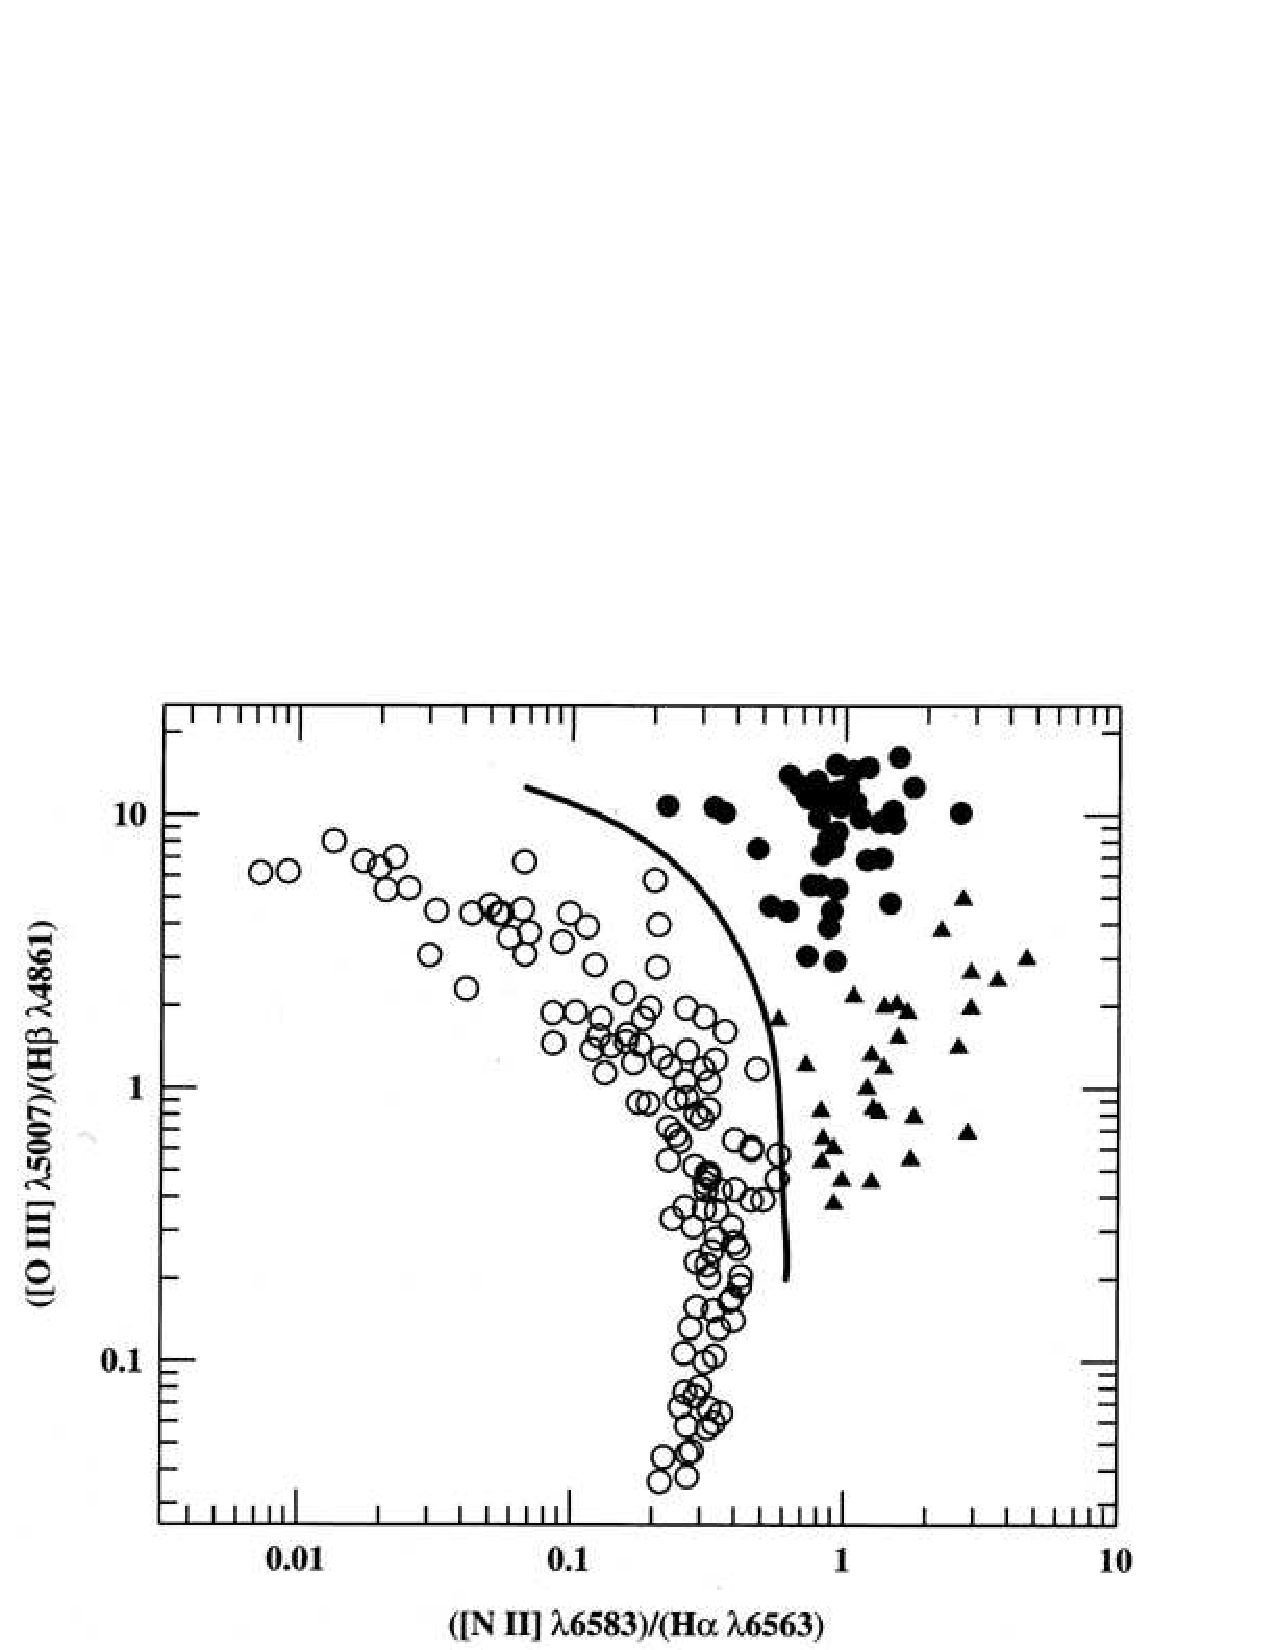
\includegraphics[height=8.0cm,width=6.0cm]
      {BPT.pdf}
      \caption[]{}
    \end{figure}
    [O III]/[O II] is sensitive to ionization parameter (how ionized is the gas).
    [O I]/ H $\alpha$ is sensitive to hardness of the radiation field. 
    
    
\section{C}

    \subsection{Covering Factor}
    From \citet[e.g.,][]{Roseboom13}...
``The fraction of sight-lines to the AGN centre obscured by dust.''

    \subsection{Comption Thick}
    Straight from: \href{http://ned.ipac.caltech.edu/level5/March04/Comastri/frames.html}{Comastri,  astro-ph/0403693}.
    
    The spectrum of the hard X-ray background records the history of
    accretion processes integrated over the cosmic time. Several pieces of
    observational and theoretical evidence indicate that a significant
    fraction of the energy density is obscured by large columns of gas and
    dust. The absorbing matter is often very thick, {\bf with column densities
      exceeding $N_{\rm H} \simeq 1.5 \times10^{24}$ cm$^{-2}$, the value corresponding to unity
      optical depth for Compton scattering}. These sources are called
    "Compton thick" and appear to be very numerous, at least in the nearby
    universe. Although Compton thick Active Galactic Nuclei (AGN) are
    thought to provide an important contribution to the overall cosmic
    energy budget, their space density and cosmological evolution are
    poorly known. The properties of Compton thick AGN are reviewed here,
    with particular emphasis on their contributions to the extragalactic
    background light in the hard X-ray and infrared bands.
    
\section{D}
    \subsection{Duty cycle}
    ``the fraction of the time that an AGN/QSO is active.''


\section{L}
\subsection{LINERS}
Straight from Sturm et al., 2006, ApJL, 653, L13:\\
Since their identification as a class of galactic nuclei more than 25
years ago (Heckman 1980), the nature of low-ionization nuclear
emission-line regions (LINERs) has remained controversial. Their
optical spectra are characterized by enhanced narrow emission lines
of low-ionization species, quite distinct from those of both {H~\sc{ii}} 
regions and classical active galactic nuclei (AGNs). They are found in
one-third to one-half of all types nearby galaxies (e.g., Ho et
al. 1997). In many LINERs the emission is concentrated near the
nucleus (a few times 100 pc; e.g., Pogge et al. 2000), but in others
it extends over larger regions, up to a few kiloparsecs (Veilleux et
al. 1995). There is substantial evidence that many LINERs are powered
by accretion onto massive black holes and that these objects, due to
low accretion rates, constitute the low-luminosity end of the AGN
class (Quataert 2001; Kewley et al. 2006). If many LINERs at low and
high redshifts are indeed low-luminosity AGNs, this would have a
significant impact on major issues in astronomy such as the growth
history of central black holes and the relation of AGNs to galaxy
formation and evolution.

\section{R}
\subsection{Reddening}

\section{S}
\subsection{Salpeter time}
\begin{equation}
  t_{S} = M/\dot{M} = 4.5 \times10^{7} \left( \frac{\epsilon}{0.1}\right ) \left( \frac{L}{L_{\rm Edd}}\right )^{-1}
\end{equation}
where $\epsilon = L/\dot{M} c^{2}$ is the radiative efficiency for a QSO radiating at a fraction $L/LEdd$ of the Eddington luminosity. Commonly accepted values of these two key parameters for luminous QSOs are $\epsilon= 0.1$ and $L/LEdd = 1$. 
Martini, P. (QSO Lifetimes; http://adsabs.harvard.edu/abs/2004cbhg.symp..169M). 

This critical accretion rate, [the Eddington mass accretion rate], is proportional to the mass of the accreting object, which implies that the mass of an object that is growing at the maximal (Eddington) accretion grows exponentially on a timescale known as the Salpeter time,
\begin{equation}
  t_{Sal} = \frac{\epsilon \sigma_{T} c}{4\pi G m_{p}} \approx 45 \epsilon_{0.1} 10^6 \, {\rm years}
\end{equation}
from ``Massive Black Hole Growth and Formation'' from Paolo Coppi. 
%%tSal = εσT c ≈ 45ε0.1106 years, (1) 4πGmp


\subsection{Soltan Argument}
\begin{equation}
  \frac{\epsilon}{1-\epsilon} \, \rho_{\rm BH} c^{2} = \int e(z) (1+z) dz
\end{equation}
$e(z) dz$ : present energy density from AGN in redshift range $z$ to $z+dz$.\\
$\rho_{\rm BH}$: mean cosmic density of nuclear black holes.\\
$\eta$: radiative efficiency\\
The Soltan argument works approximately for $\eta\approx$0.1, 
so observed AGN must account for most of nuclear black hole growth.

Refs:\\
www.aei.mpg.de/~pau/conf\_vid/Miralda.pdf\\
www.bo.astro.it/~vignali/PhD.../Merloni\_PhD\_Bologna\_Tuesday.pptx
www.astro.yale.edu/coppi/pubs/bhgrowth4.pdf
http://ned.ipac.caltech.edu/level5/March02/Ferrarese/Fer2.html

\section{T} 
\subsection{Thomson cross-section}
$N_{\rm H} \geq \sigma_{\rm T}^{-1} \simeq 1.5 \times 10^{24}$ cm$^{-2}$. 
%http://ned.ipac.caltech.edu/level5/March04/Comastri/Comastri1.html

For an electron:
\begin{equation}
\sigma_{\rm T}= \frac{8\pi}{3} \left(\frac{\alpha\hbar c}{mc^2}\right)^2 = 0.6652\times10^{-24} \,\, \rm{cm}^{-2}
\end{equation}

\subsection{Thomson scattering} 
%%http://en.wikipedia.org/wiki/Thomson_scattering
Thomson scattering is the elastic scattering of electromagnetic radiation by a free charged particle. It is just the low-energy limit of Compton scattering: the particle kinetic energy and photon frequency are the same before and after the scattering. This limit is valid as long as the photon energy is much less than the mass energy of the particle: $\nu\ll mc^2/h$.

\bibliographystyle{mn2e}
\bibliography{/cos_pc19a_npr/LaTeX/tester_mnras}

\end{document}

